\clearpage % guidance only
\section{Bias} \label{sec:unfolding:bias}
As explained in \autoref{sec:dsea:dsea},
\dsea{} is intended to eliminate the bias introduced by the energy spectrum of the Monte Carlo training data.
%
In order to test
whether the bias is indeed eliminated,
the model is evaluated on a \emph{stratified} data set,
    where each bin contains an equal number of events,
whereas the training data is the same as before.
% NOTE: This stratified test data set is smaller than its unstratified counterpart,
% because I stratify AFTER bootstrapping.
% About 1000 events per bin remain.
%
% COULDDO: Samuel did the opposite: stratified training data, but not test data. I should consider doing the same. (@Leonora)

The results are shown in \autoref{fig:bias_comparison}.
As can be seen,
The model adapts to the unseen distribution of the test data.
No significant amount of bias is observed.
In comparison to the unfolding of unmodified test data in \autoref{fig:bootstrap:spectrum},
the relative deviations are even smaller on average.
%
% COULDDO: Move to summary?
For comparison,
in the work by \citeauthor{dsea_samuel} \cite{dsea_samuel},
  where the training data is stratified
    instead of the test data,
relative deviations of more than \SI{1500}{\percent} are observed.
% Aber er schiebt's auf die geringe Accuracy…


\begin{figure}
  \centering
  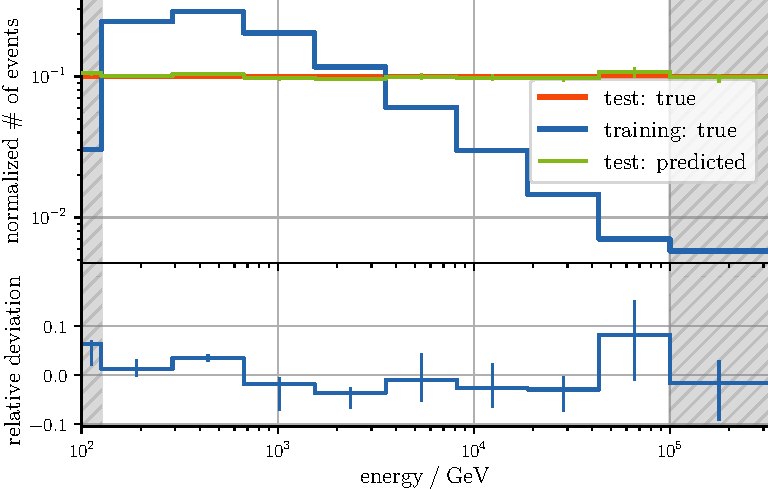
\includegraphics[scale=1]{content/plots/bias:spectrum_full.pdf}
  \caption{
    Energy spectrum and relative deviations of a bootstrap run
    on a stratified test data set.
  }
  \label{fig:bias_comparison}
\end{figure}
